\newpage
\null
\thispagestyle{empty}
\newpage
\addcontentsline{toc}{chapter}{Jonah}


% Safely inserts your illustration full-bleed on its own page.
% This completely bypasses the page builder, headers, and geometry bugs!
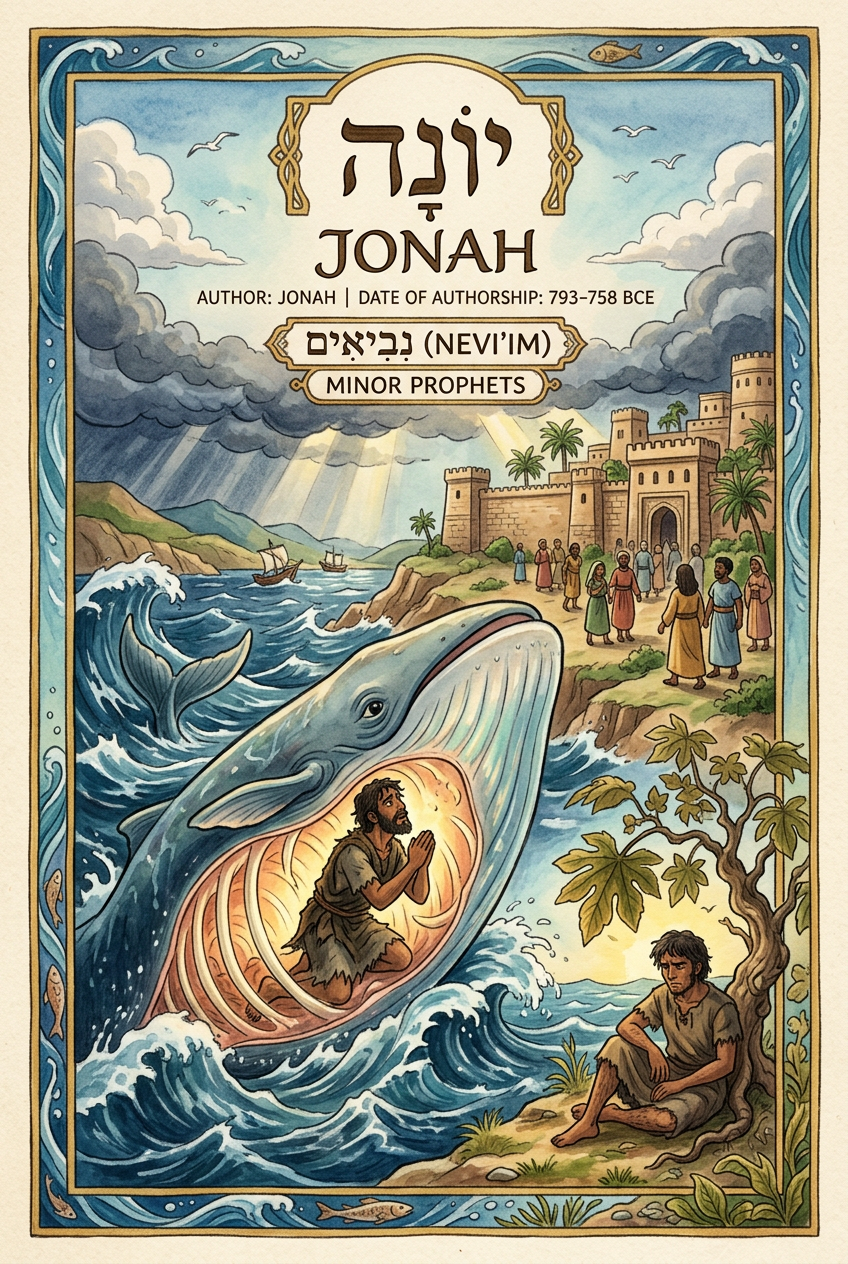
\includepdf[pages=1, fitpaper=false, width=\paperwidth, height=\paperheight, , keepaspectratio=false]{images/divider2/jonah_2.png}
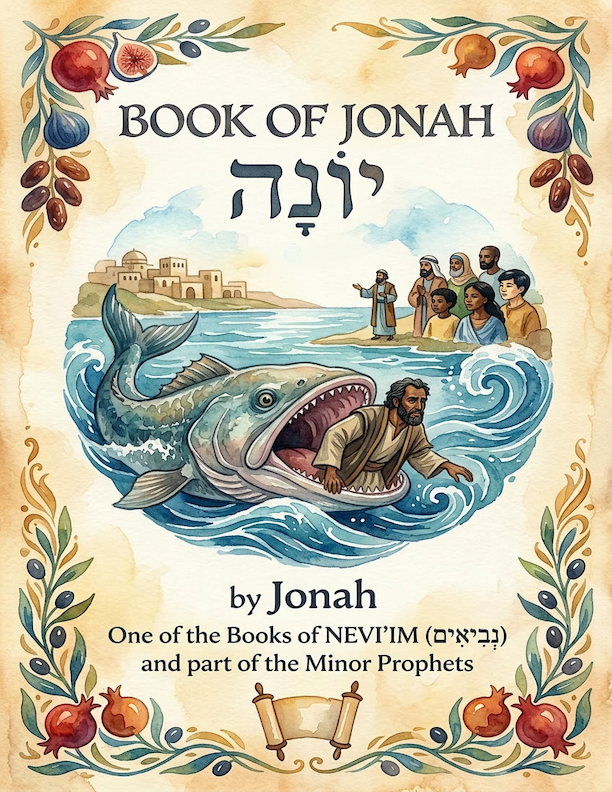
\includepdf[pages=1, fitpaper=false, width=\paperwidth, height=\paperheight, , keepaspectratio=false]{images/divider1/jonah.png}

\includepdf[pages=1, fitpaper=false, width=\paperwidth, height=\paperheight, , keepaspectratio=false]{images/8.5x11-Dot-Grid.png}

\includepdf[pages=1, fitpaper=false, width=\paperwidth, height=\paperheight, , keepaspectratio=false]{images/8.5x11-Dot-Grid.png}
\mybook{Jonah}
\vspace{-1.36in}

\mychapter{} \myverse*{}Now the LORD’s\footnote{1:1 When rendered in ALL CAPITAL LETTERS, “LORD” or “GOD” is the translation of God’s Proper Name.}
word came to Jonah the son of Amittai, saying,
\myverse{}“Arise, go to Nineveh, that great city, and proclaim against it, for their wickedness
has come up before me.”

\myverse{}But Jonah rose up to flee to Tarshish from the presence of the
LORD. He went down to Joppa, and found a ship going to Tarshish; so he paid its fare, and went down into
it, to go with them to Tarshish from the presence of the LORD.

\myverse{}But the LORD sent out a great wind on the sea, and there was a
mighty storm on the sea, so that the ship was likely to break up.
\myverse{}Then the mariners were afraid, and every man cried to his god. They threw the
cargo that was in the ship into the sea to lighten the ship. But Jonah had gone down into the innermost
parts of the ship and he was laying down, and was fast asleep.
\myverse{}So the ship master came to him, and said to him, “What do you mean, sleeper?
Arise, call on your God!\footnote{1:6 or, gods} Maybe your God\footnote{1:6 or, gods
} will notice us, so that we won’t perish.”

\myverse{}They all said to each other, “Come! Let’s cast lots, that we may
know who is responsible for this evil that is on us.” So they cast lots, and the lot fell on Jonah.
\myverse{}Then they asked him, “Tell us, please, for whose cause this evil is on us. What
is your occupation? Where do you come from? What is your country? Of what people are you?”

\myverse{}He said to them, “I am a Hebrew, and I fear the LORD, the God\footnote{1:9 The Hebrew word rendered “God” is “אֱלֹהִ֑ים” (Elohim).} of heaven, who has
made the sea and the dry land.”

\myverse{}Then the men were exceedingly afraid, and said to him, “What
have you done?” For the men knew that he was fleeing from the presence of the LORD, because he had told
them.
\myverse{}Then they said to him, “What shall we do to you, that the sea may be calm
to us?” For the sea grew more and more stormy.

\myverse{}He said to them, “Take me up, and throw me into the sea. Then
the sea will be calm for you; for I know that because of me this great storm is on you.”

\myverse{}Nevertheless the men rowed hard to get them back to the land;
but they could not, for the sea grew more and more stormy against them.
\myverse{}Therefore they cried to the LORD, and said, “We beg you, LORD, we beg you,
don’t let us die for this man’s life, and don’t lay on us innocent blood; for you, LORD, have done as
it pleased you.”
\myverse{}So they took up Jonah and threw him into the sea; and the sea ceased its raging.
\myverse{}Then the men feared the LORD exceedingly; and they offered a sacrifice to
the LORD and made vows.

\myverse{}The LORD prepared a huge fish to swallow up Jonah, and Jonah
was in the belly of the fish three days and three nights.


%JONAH 2
\mychapter{} \myverse*{}Then Jonah prayed to the LORD, his God, out of the fish’s belly.
\myverse{}He said,

“I called because of my affliction to the LORD.

He answered me.

Out of the belly of Sheol\footnote{2:2 Sheol is the place of the dead.} I cried.

You heard my voice.

\myverse{}For you threw me into the depths,

in the heart of the seas.

The flood was all around me.

All your waves and your billows passed over me.

\myverse{}I said, ‘I have been banished from your sight;

yet I will look again toward your holy temple.’

\myverse{}The waters surrounded me,

even to the soul.

The deep was around me.

The weeds were wrapped around my head.

\myverse{}I went down to the bottoms of the mountains.

The earth barred me in forever;

yet you have brought my life up from the pit, LORD my God.


\vspace{\baselineskip} \myverse{}“When my soul fainted within me, I remembered the LORD.

My prayer came in to you, into your holy temple.

\myverse{}Those who regard vain idols forsake their own mercy.

\myverse{}But I will sacrifice to you with the voice of thanksgiving.

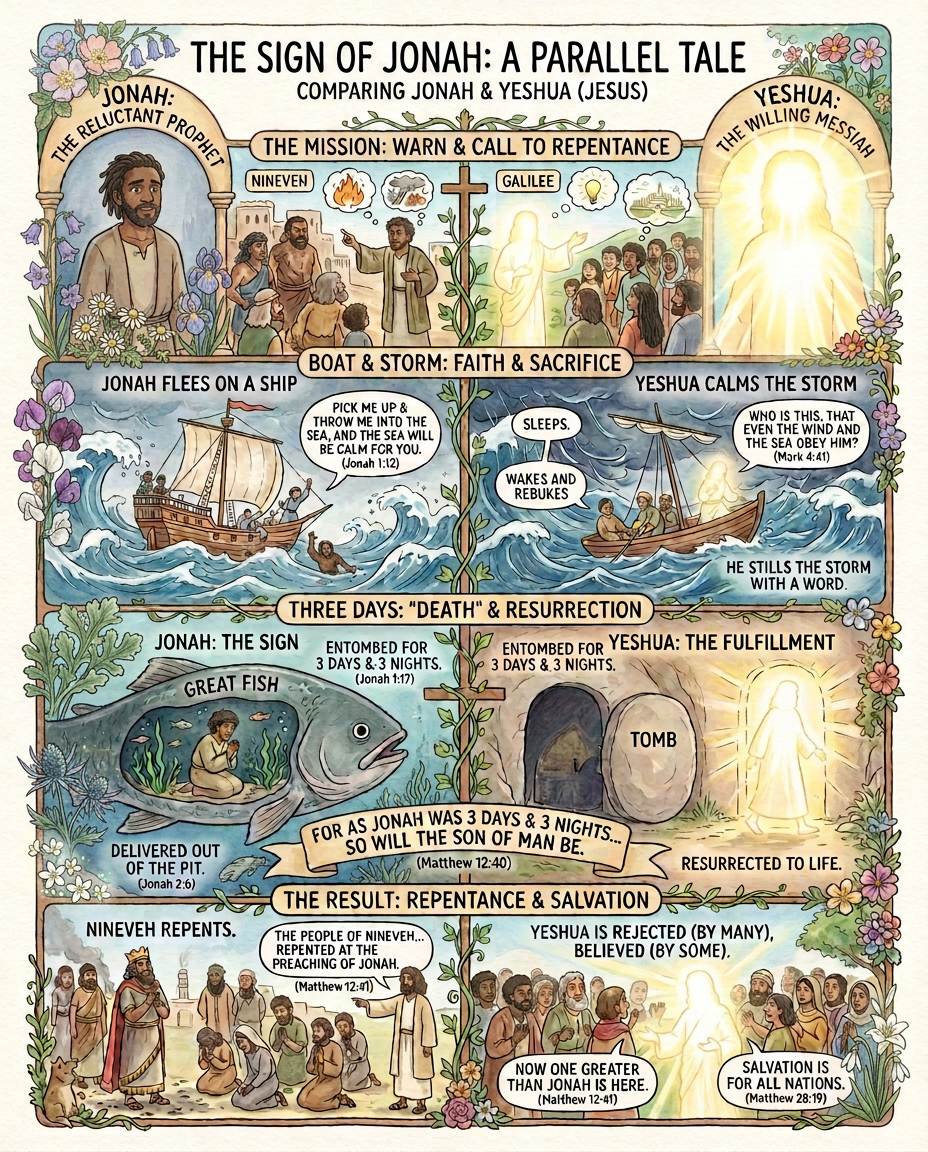
\includepdf[pages=1, fitpaper=false, width=\paperwidth, height=\paperheight, , keepaspectratio=false]{jonah-comparison.png}

\noindent I will pay that which I have vowed.

Salvation belongs to the LORD.”

\myverse{}Then the LORD spoke to the fish, and it vomited out Jonah on
the dry land.


%JONAH 3
\mychapter{} \myverse*{}The LORD’s word came to Jonah the second time, saying,
\myverse{}“Arise, go to Nineveh, that great city, and proclaim to it the message that
I give you.”

\myverse{}So Jonah arose, and went to Nineveh, according to the LORD’s word.
Now Nineveh was an exceedingly great city, three days’ journey across.
\myverse{}Jonah began to enter into the city a day’s journey, and he cried out, and said,
“In forty days, Nineveh will be overthrown!”

\myverse{}The people of Nineveh believed God; and they proclaimed a fast
and put on sackcloth, from their greatest even to their least.
\myverse{}The news reached the king of Nineveh, and he arose from his throne, took off
his royal robe, covered himself with sackcloth, and sat in ashes.
\myverse{}He made a proclamation and published through Nineveh by the decree of the king
and his nobles, saying, “Let neither man nor animal, herd nor flock, taste anything; let them not feed,
nor drink water;
\myverse{}but let them be covered with sackcloth, both man and animal, and let them cry
mightily to God. Yes, let them turn everyone from his evil way and from the violence that is in his hands.
\myverse{}Who knows whether God will not turn and relent, and turn away from his fierce
anger, so that we might not perish?”

\myverse{}God saw their works, that they turned from their evil way. God
relented of the disaster which he said he would do to them, and he didn’t do it.


%JONAH 4
\mychapter{} \myverse*{}But it displeased Jonah exceedingly, and he was angry.
\myverse{}He prayed to the LORD, and said, “Please, LORD, wasn’t this what I said when
I was still in my own country? Therefore I hurried to flee to Tarshish, for I knew that you are a gracious
God and merciful, slow to anger, and abundant in loving kindness, and you relent of doing harm.
\myverse{}Therefore now, LORD, take, I beg you, my life from me, for it is better for
me to die than to live.”

\myverse{}The LORD said, “Is it right for you to be angry?”

\myverse{}Then Jonah went out of the city and sat on the east side of the
city, and there made himself a booth and sat under it in the shade, until he might see what would become
of the city.
\myverse{}The LORD God prepared a vine and made it to come up over Jonah, that it might
be a shade over his head to deliver him from his discomfort. So Jonah was exceedingly glad because of
the vine.
\myverse{}But God prepared a worm at dawn the next day, and it chewed on the vine so that
it withered.
\myverse{}When the sun arose, God prepared a sultry east wind; and the sun beat on Jonah’s
head, so that he was faint and requested for himself that he might die. He said, “It is better for me
to die than to live.”

\myverse{}God said to Jonah, “Is it right for you to be angry about the vine?”

He said, “I am right to be angry, even to death.”

\myverse{}The LORD said, “You have been concerned for the vine, for which
you have not labored, neither made it grow; which came up in a night and perished in a night.
\myverse{}Shouldn’t I be concerned for Nineveh, that great city, in which are more than
one hundred twenty thousand persons who can’t discern between their right hand and their left hand, and
also many animals?”


